\subsection{Example Walkthrough}
\label{sub:walk}

The following subsection describes a walkthrough for a new analysis involving a sample data set provided by I. Sassoon (see \autoref{app:dataset}) and a survival analysis by gender (preferences set according to \cite{sassoon2016CD}). These initial options are selected in \autoref{fig:analysis:1}. The following screen (see \autoref{fig:analysis:2}) shows the actual analysis screen. All \texttt{TestAssumptions} have already been evaluated and on the left hand side of the screenshot the \textit{Currently Possible Models} are depicted. On the right hand side the \textit{Open Query Assumptions} are presented to the user including one \texttt{QueryTestAssumption} with a generated plot for this particular data set and one \texttt{QueryAssumption}. 

\begin{figure}[b]
	\centering
	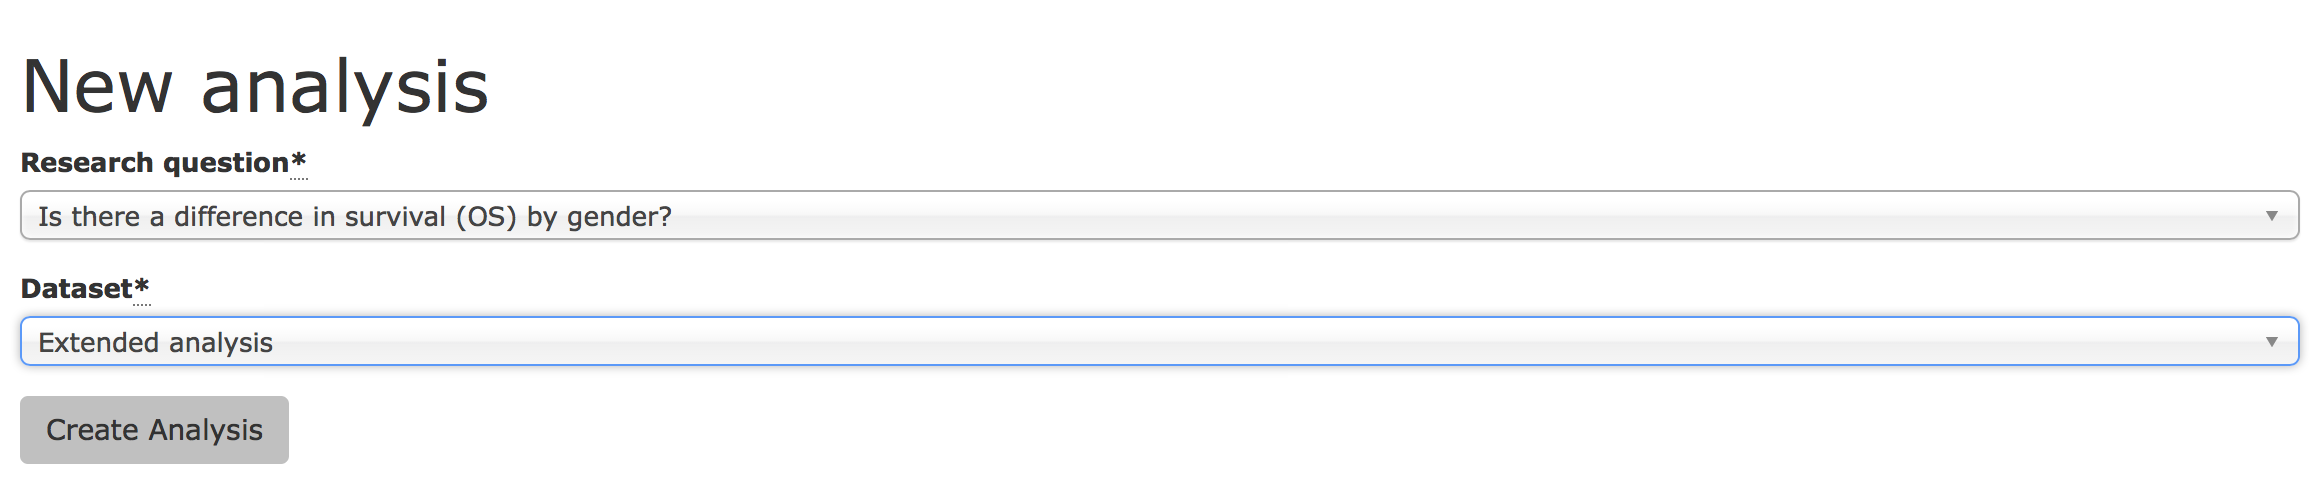
\includegraphics[width=\textwidth]{figures/ui_analysis_0}
	\caption{Creating a new analysis, step 1: Selection of a data set and research question. }
	\label{fig:analysis:1}
\end{figure}

In this particular case, all entered models for the given research question are possible. If one \texttt{TestAssumption} for one of those models would not hold and this model would have further \texttt{Query(Test)Assumptions}, these will not be presented to the end-user, as this model is already not possible anymore. If multiple models require the same answers to one \texttt{QueryAssumption} (e.g. for our example all three models depend on assumption \texttt{A1}) the clinician will only be asked to answer this question once. 

\begin{figure}[t]
	\centering
	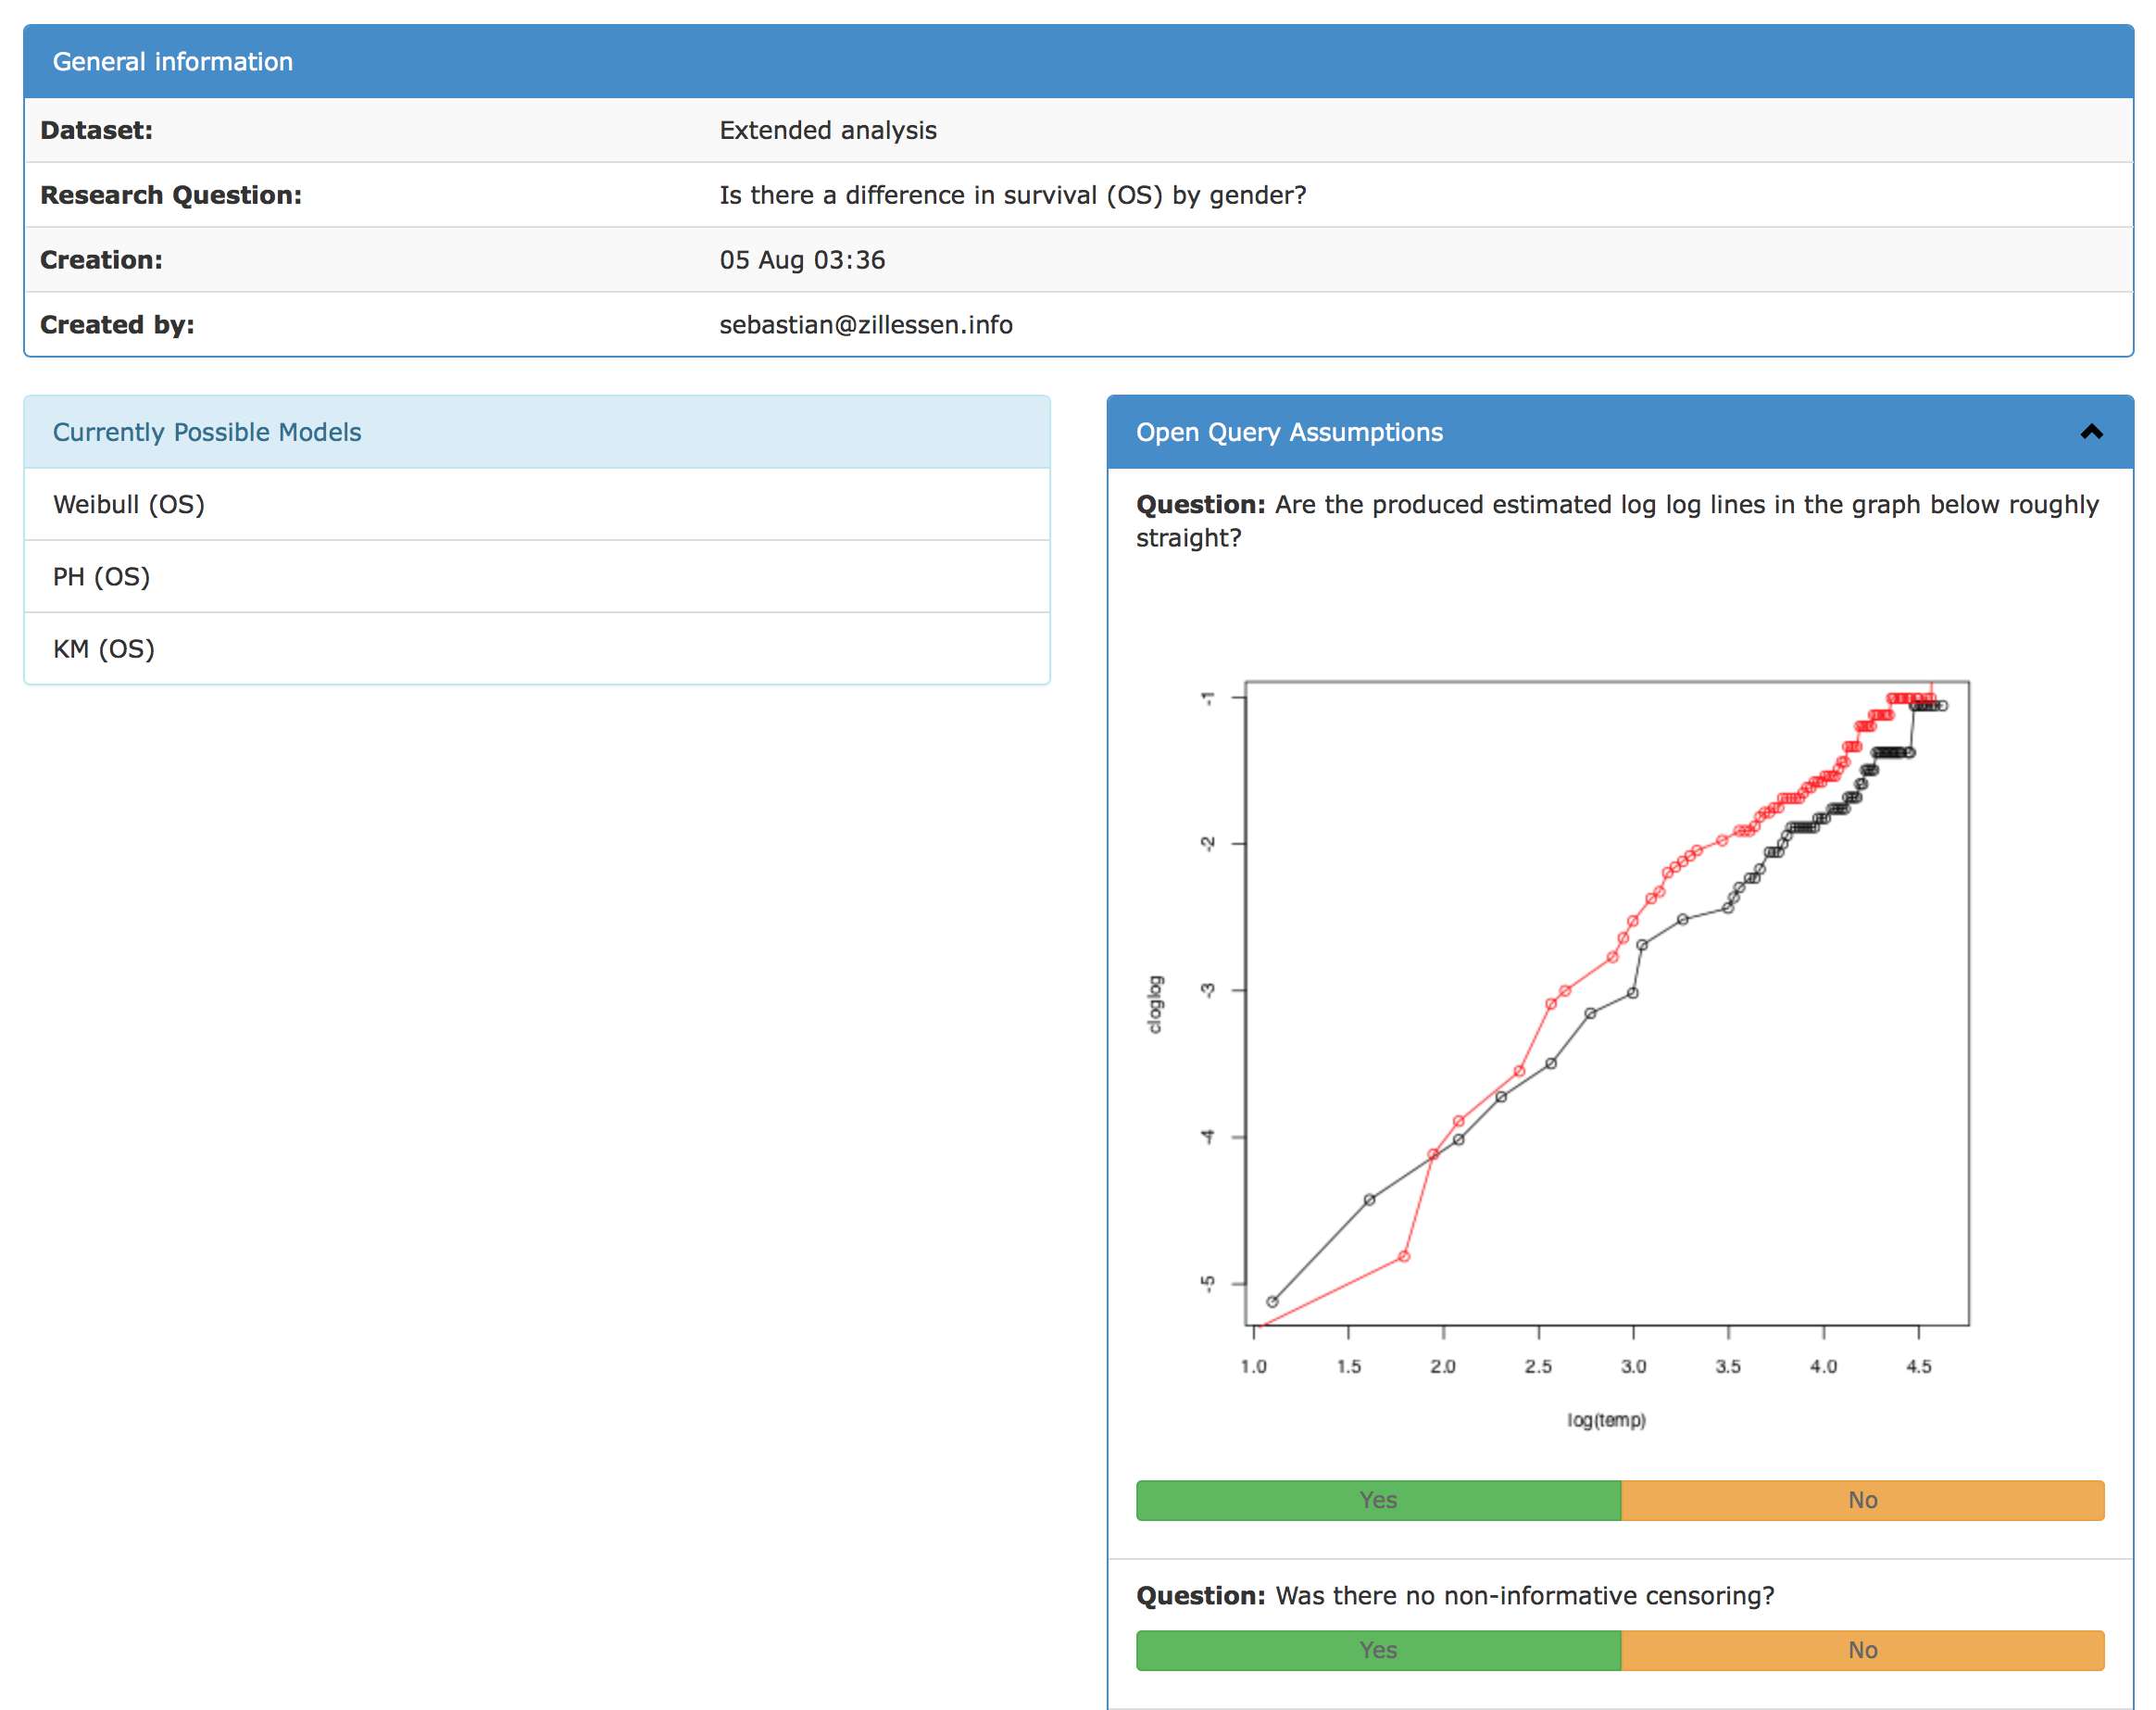
\includegraphics[width=\textwidth]{figures/ui_analysis_1}
	\caption{Creating a new analysis, step 2: Clinician has to answer \texttt{QueryTest-} and \texttt{QueryAssumptions} to perform the analysis. \texttt{TestAssumptions} have already been evaluated.}
	\label{fig:analysis:2}
\end{figure}


As soon as the clinician answers one of the \texttt{QueryAssumptions} the analysis will be updated according to this answer and if some of the \texttt{QueryAssumptions} that are already visible to the user get obsolete by this answer, they will be removed from the open- and moved to the ignored-list (right lower part of \autoref{fig:analysis:3_no}). 
As the clinician answered \texttt{A1} with \textit{No}, the analysis results in no possible models, so no preferences are employed and the analysis is finished.

\begin{figure}[t]
	\centering
	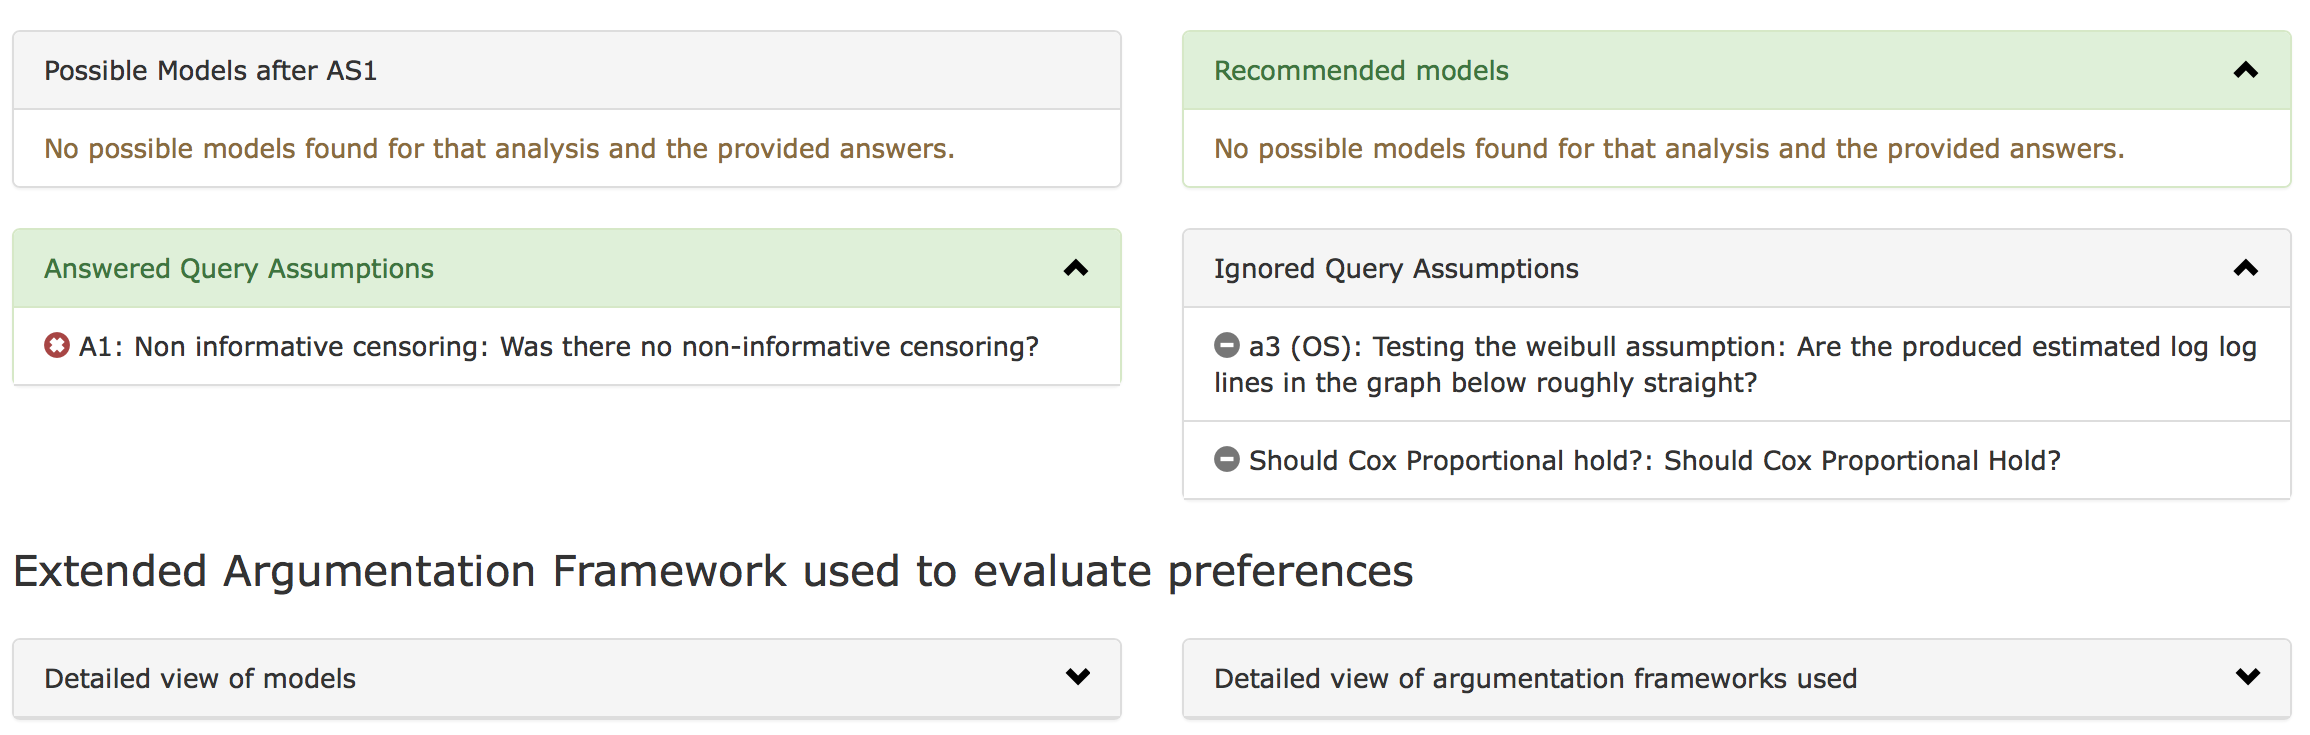
\includegraphics[width=\textwidth]{figures/ui_analysis_2_no}
	\caption{Creating a new analysis, step 3: After answering one question (e.g. "A1: Has no non-informative censoring been in place?" with \textit{No}), the possible models are updated and outdated \texttt{QueryAssumptions} are moved from the list of queries to the list of \textit{Ignored Query Assumptions}.}
	\label{fig:analysis:3_no}
\end{figure}

However, if all \texttt{QueryAssumptions} have been answered positively all three models remain possible. The system will now initiate the \gls{EAF} for this particular analysis as described in \autoref{sub:statistical_model_selection}. The evaluation of this \gls{EAF} is performed in the same order: First, the \texttt{TestAssumptions} are evaluated. Second, if no final solution of the \gls{EAF} could be found, the \texttt{Query(Test)Assumptions} required for the first preference are evaluated. This process is then repeated with the remaining preferences and their \glspl{CD}.

\begin{figure}[t]
	\centering
	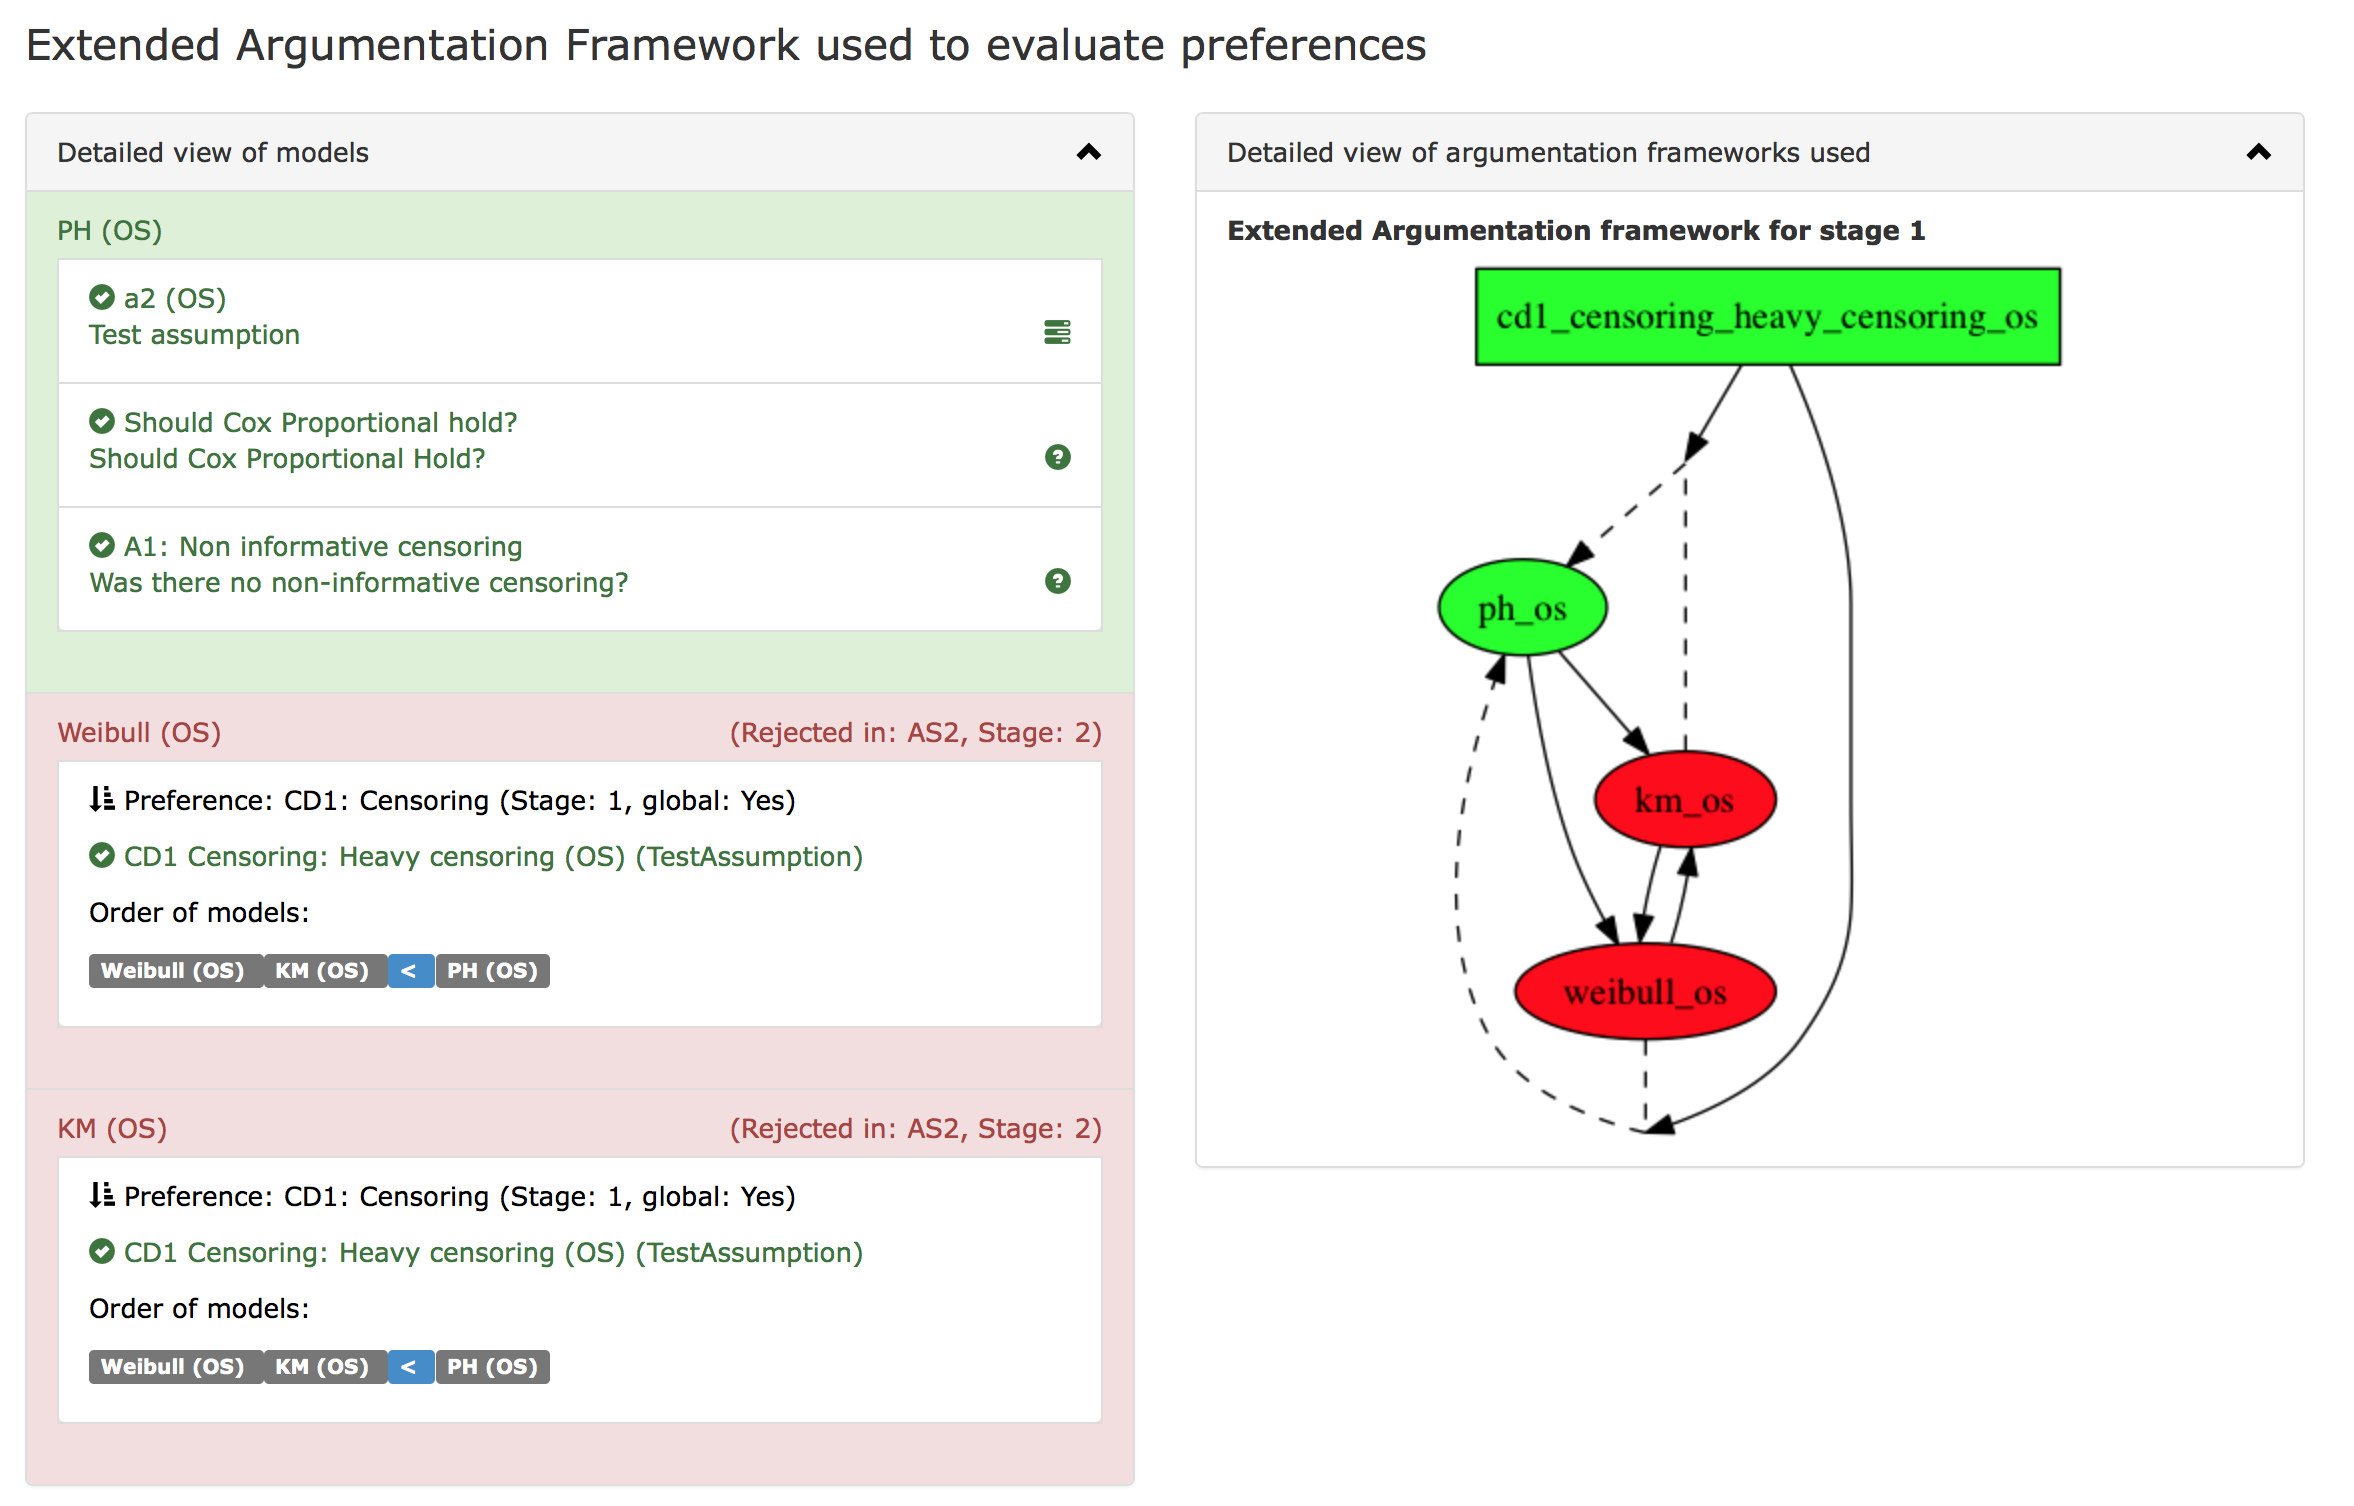
\includegraphics[width=\textwidth]{figures/ui_analysis_eaf}
	\caption{Finished analysis with applied preferences on it: context domain "Censoring" evaluated to \textit{heavy censoring}. }
	\label{fig:analysis:eaf}
\end{figure}


In this particular analysis "\textit{Censoring}" has the performance measurement \textbf{heavy}. Hence, the models \textit{Kaplan-Meier} and \textit{Weibull} are wiped-out during the evaluation of the preferences per \gls{CD}. The generated \gls{EAF} on the right side of \autoref{fig:analysis:eaf} shows the reason why only \textit{Cox-Proportional hazard} remains as the last preferred model.


During the whole process the \gls{UI} provides an interactive way of communication and as it updates its content instantly, the user gets direct feedback on his interaction. In addition, the user is not required to answer all questions in a row, the analysis will still be stored in the system and can be continued at any time. 